\clearpage
\section{Opis implementacji i funkcji aplikacji}		%4

W rozdziale opisano najważniejsze elementy zaimplementowanej aplikacji. Szczególny nacisk położono na funkcje dostępne z poziomu interfejsu operatora, ponieważ założeniem projektu było stworzenie narzędzia możliwego do obsługi bez znajomości kodu źródłowego.

\subsection{Interfejs operatora}

Interfejs aplikacji został podzielony na główne zakładki:

\begin{itemize}
\item \textbf{Podgląd kamer} -- prezentuje aktywne źródła obrazu w siatce oraz pokazuje wyniki detekcji na żywo.
\item \textbf{Konfiguracja kamer} -- pozwala dodawać, usuwać i włączać źródła obrazu.
\item \textbf{Wykryty ruch} -- zawiera historię zapisanych zdarzeń i podgląd materiału dowodowego.
\item \textbf{Ustawienia} -- umożliwia zmianę reguł alarmu, modeli, progów detekcji, archiwizacji i wzorca ubioru.
\item \textbf{Logi} -- prezentuje komunikaty diagnostyczne aplikacji oraz umożliwia ich eksport.
\end{itemize}

Główny widok aplikacji przedstawiono na rysunku \ref{fig:podglad-kamer}. Każda kamera ma osobny kafelek, na którym widoczny jest tryb pracy, liczba osób, liczba intruzów, status alarmu oraz metryki wydajności.

\begin{figure}[H]
\centering
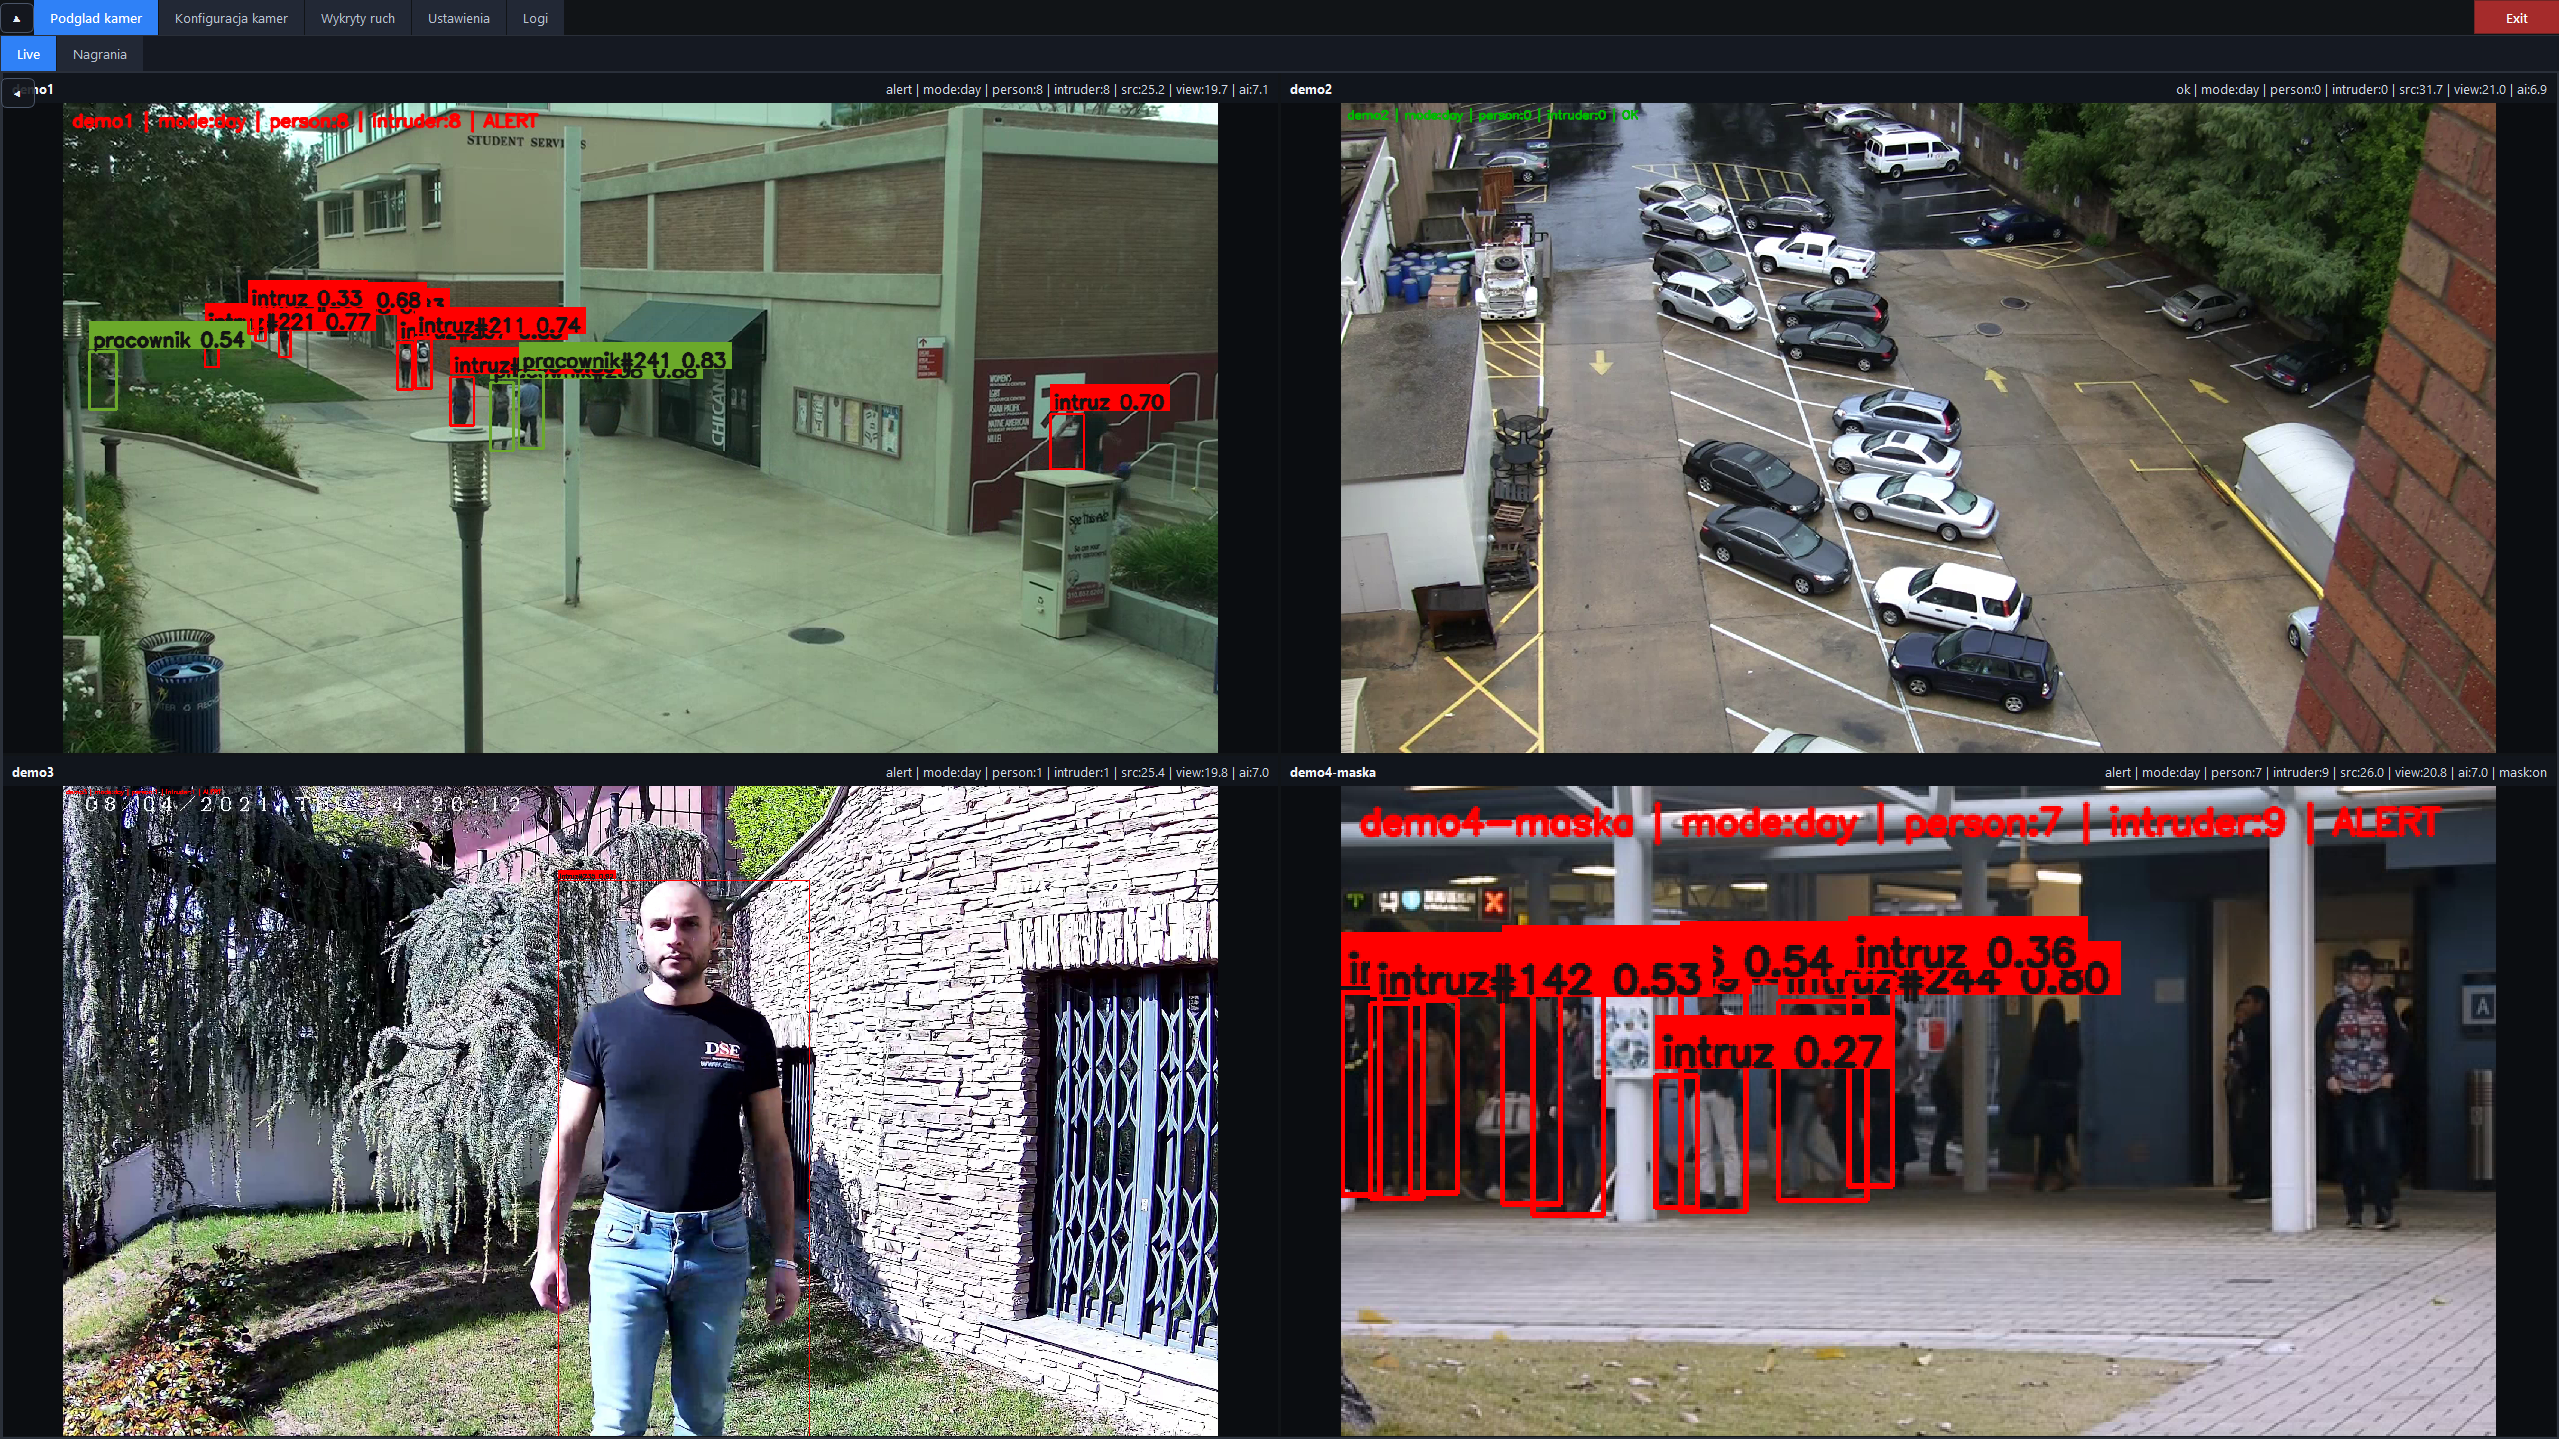
\includegraphics[width=0.95\textwidth]{rys/działanie-kamer-1.png}
\caption{Podgląd wielu źródeł obrazu z naniesionymi wynikami detekcji.}
\label{fig:podglad-kamer}
\end{figure}

\subsection{Konfiguracja źródeł obrazu}

Aplikacja obsługuje trzy typy źródeł:

\begin{itemize}
\item kamery lokalne,
\item pliki wideo,
\item strumienie sieciowe.
\end{itemize}

Operator może przeskanować dostępne kamery, dodać plik wideo, wskazać adres strumienia oraz zdecydować, które źródła mają być aktywne. Dla plików wideo dostępna jest opcja startu od losowego momentu, co ułatwia testy na nagraniach demonstracyjnych. Konfiguracja źródeł jest zapisywana w pliku ustawień aplikacji, oddzielnie od głównego pliku \texttt{inference.yaml}. Przykładowy ekran zarządzania źródłami pokazano na rysunku \ref{fig:konfiguracja-kamer}.

\begin{figure}[H]
\centering
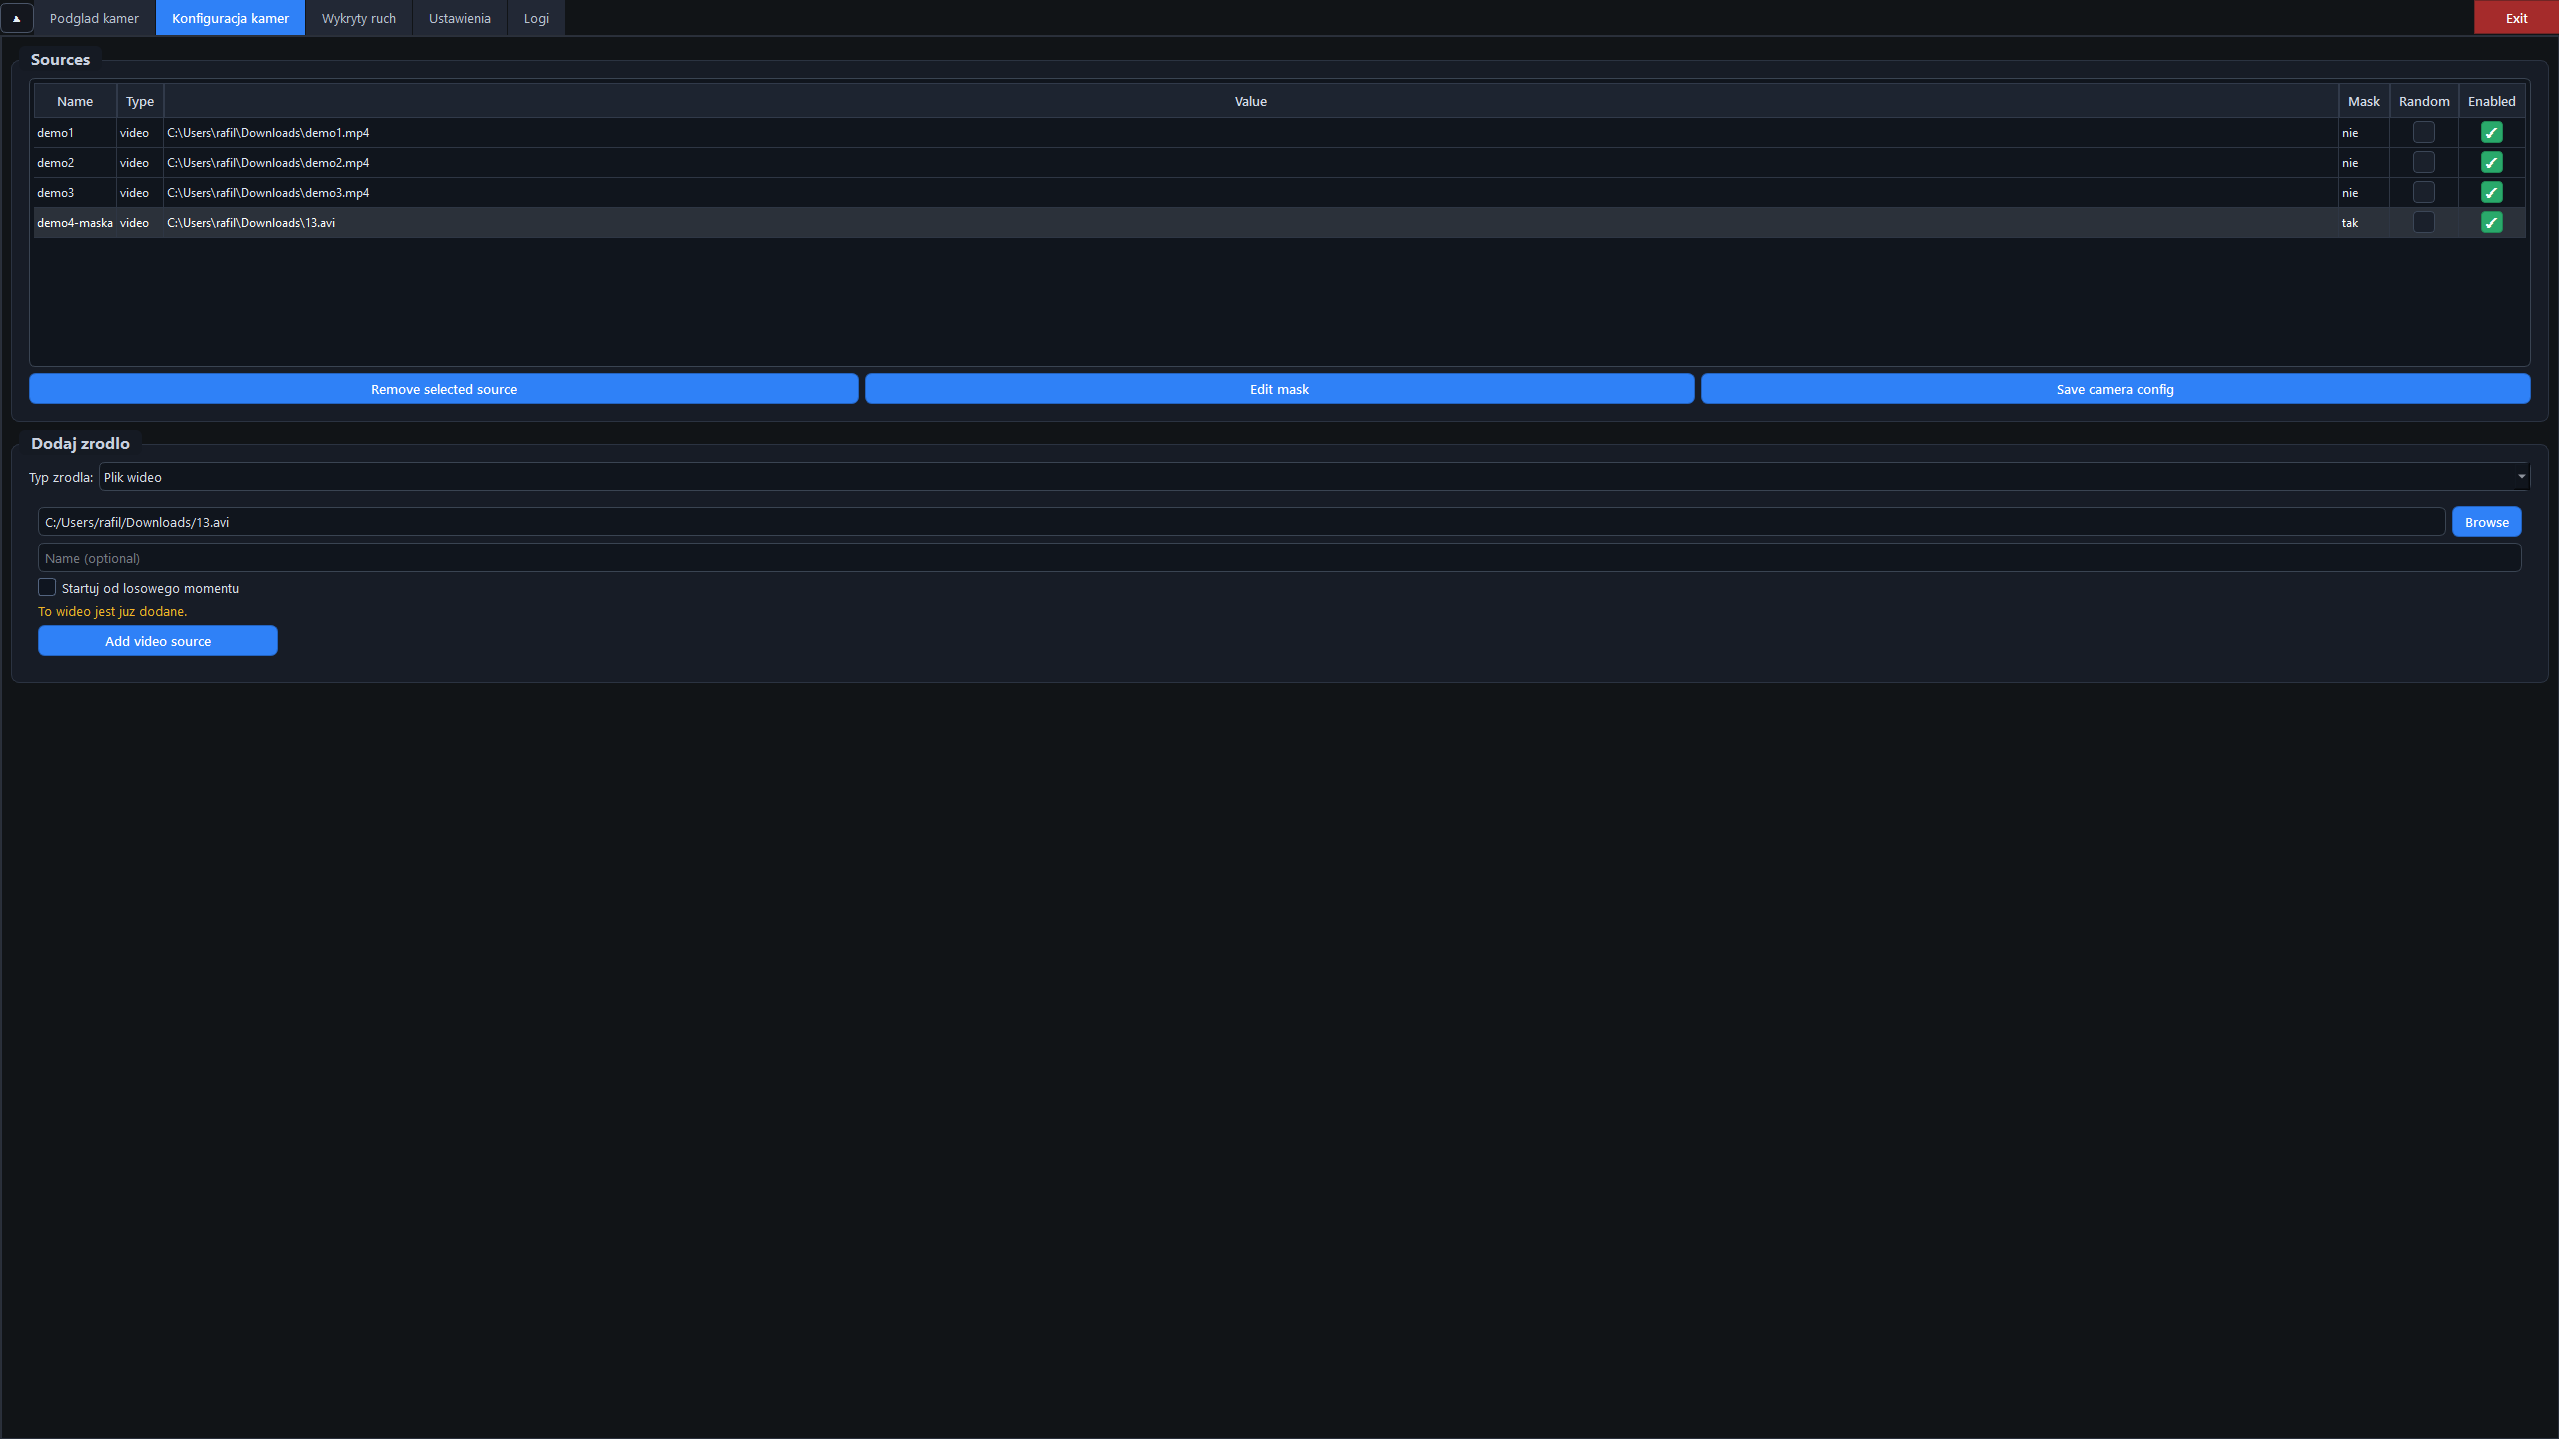
\includegraphics[width=0.95\textwidth]{rys/zakladka-konfiguracja-kamer.png}
\caption{Zakładka konfiguracji źródeł obrazu.}
\label{fig:konfiguracja-kamer}
\end{figure}

\subsection{Maski ignorowanych obszarów}

Dla każdego źródła można ustawić maskę obszaru, który ma być ignorowany przez model. Funkcja ta jest przydatna, gdy część kadru stale generuje fałszywe alarmy lub znajduje się poza obszarem zainteresowania operatora. Podczas inferencji klatka przekazywana do modelu jest modyfikowana tak, aby zamaskowany fragment nie wpływał na wyniki detekcji. Przykład działania maski widoczny jest na rysunku \ref{fig:maska}.

\begin{figure}[H]
\centering
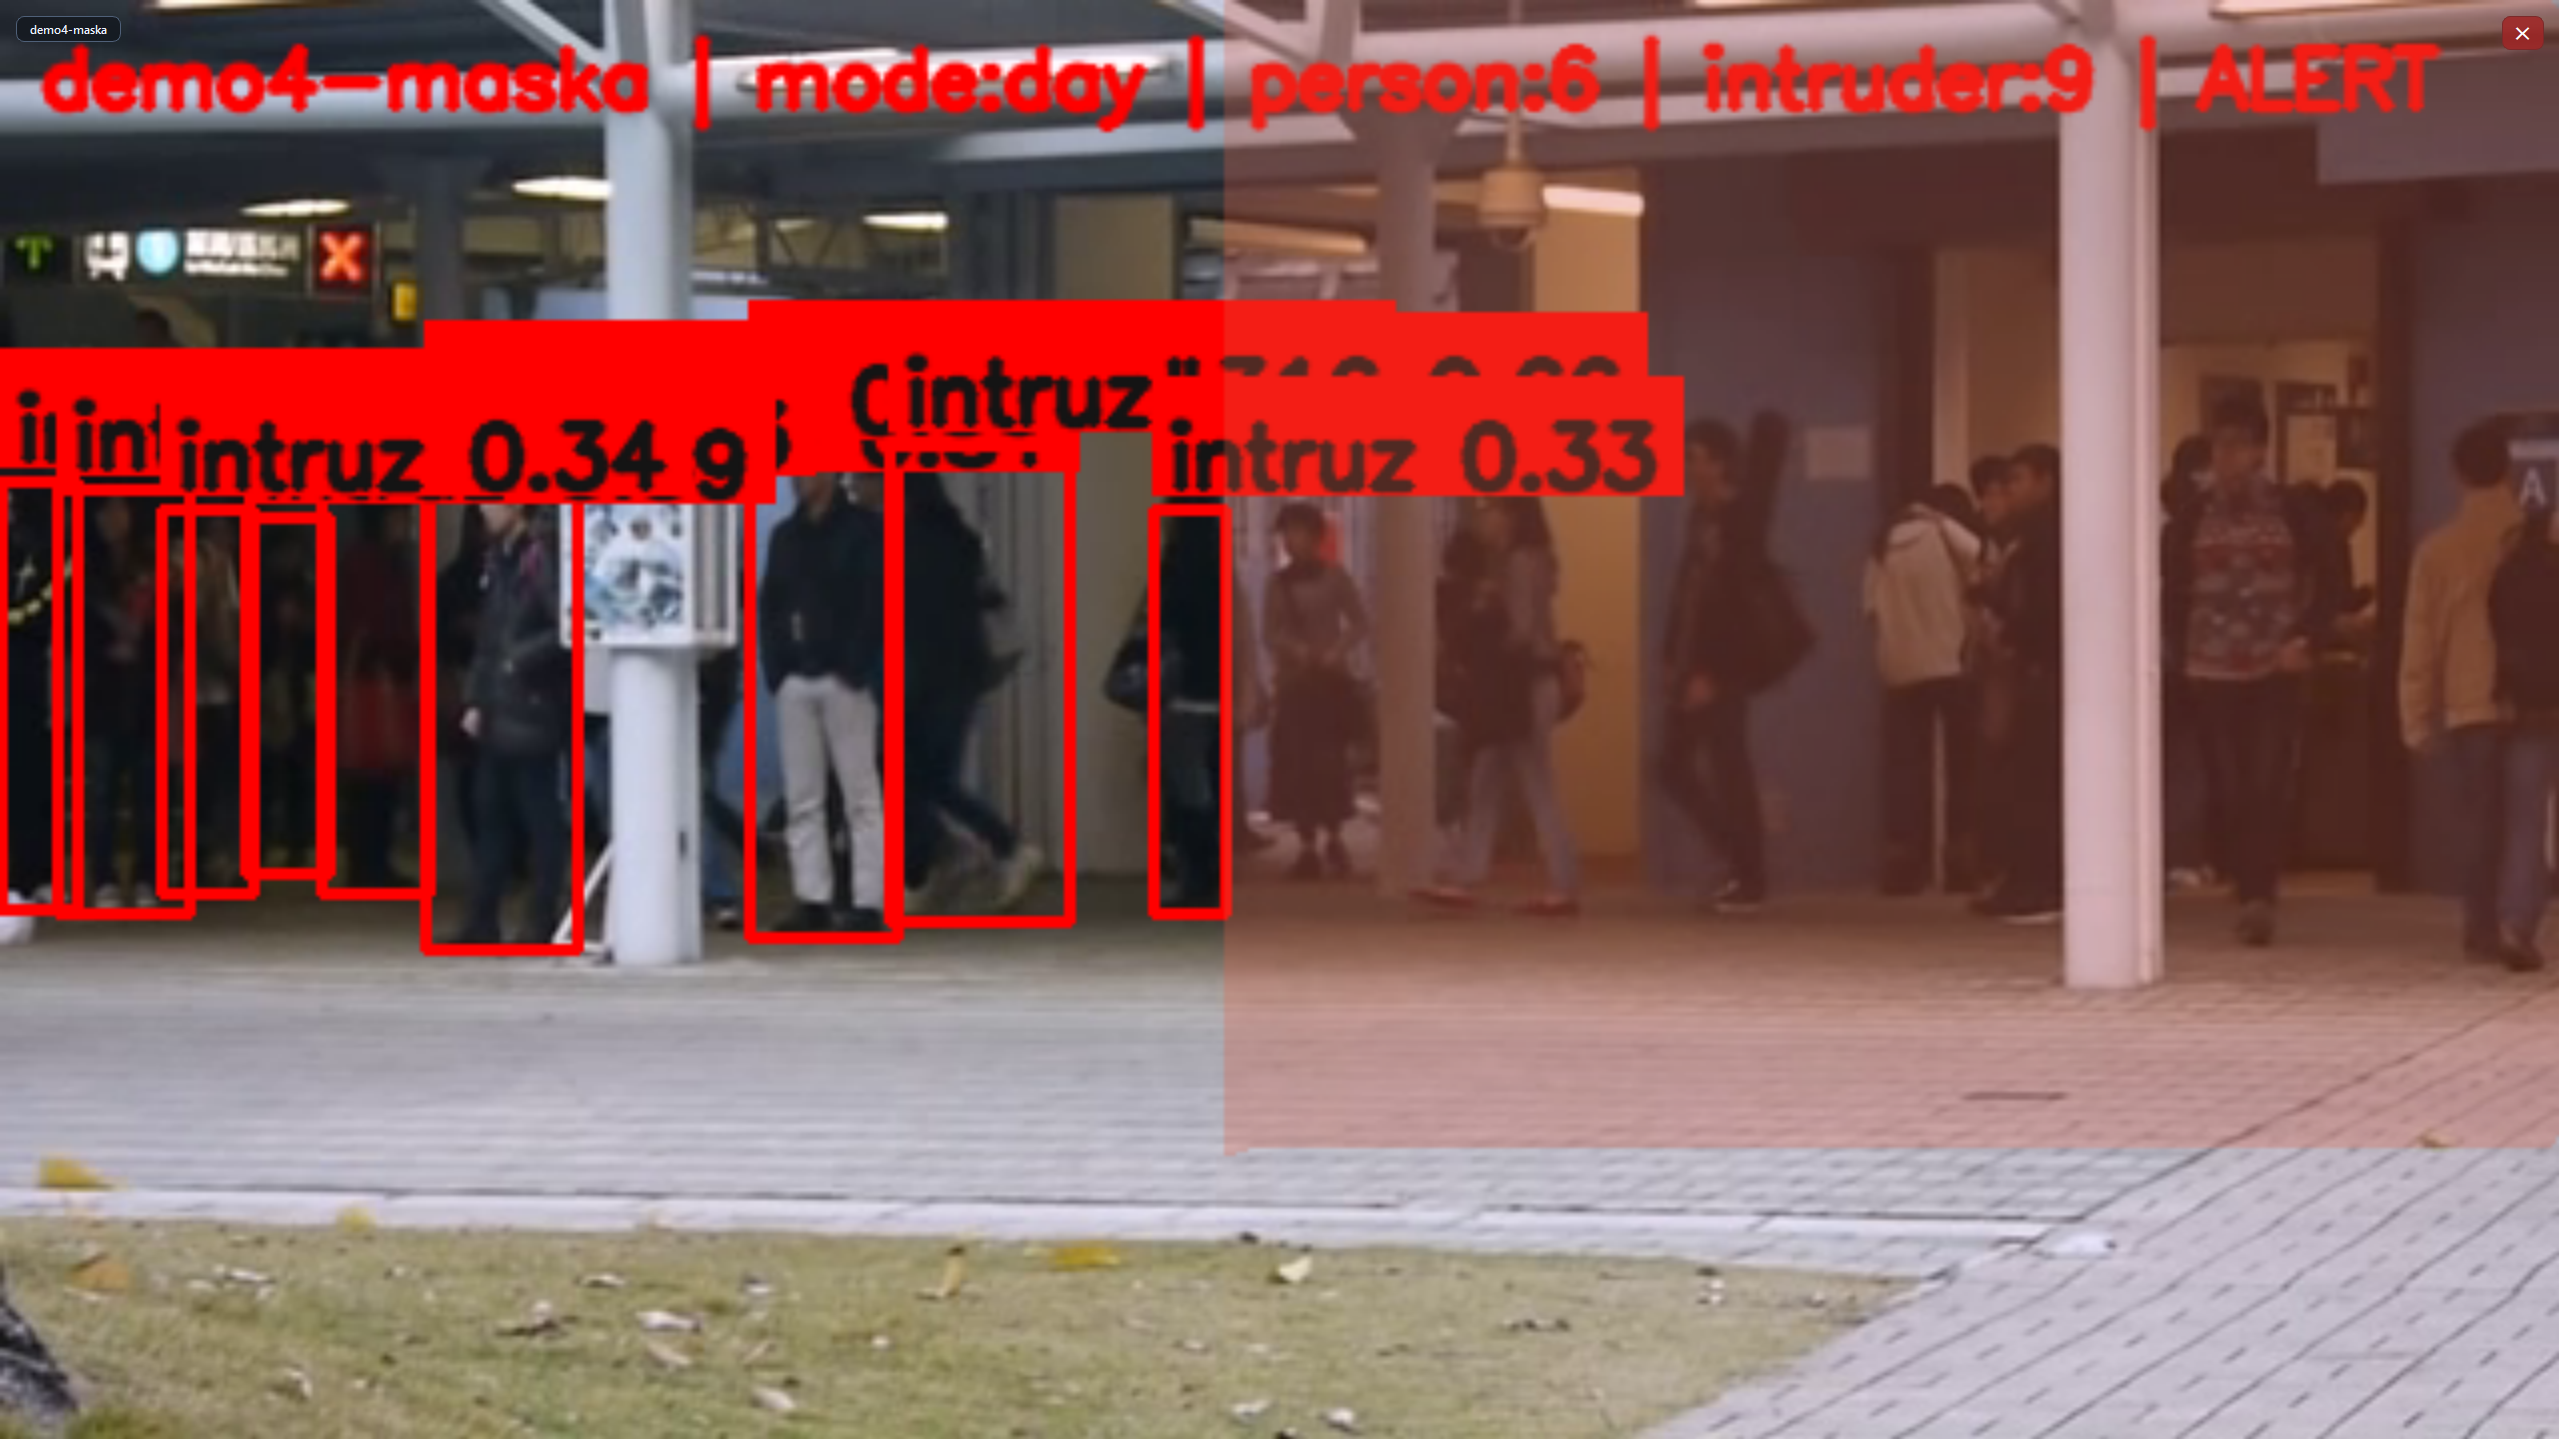
\includegraphics[width=0.95\textwidth]{rys/kamera-z-maska.png}
\caption{Przykład kamery z aktywną maską ignorowanego obszaru.}
\label{fig:maska}
\end{figure}

\subsection{Detekcja, tracking i klasyfikacja intruzów}

Detekcja osób realizowana jest przez model YOLO. Wyniki modelu są następnie przekazywane do trackera, który stabilizuje wykrycia i pozwala utrzymać ciągłość identyfikacji osoby pomiędzy klatkami. Dzięki temu etykiety na podglądzie są bardziej stabilne, a system może dokładniej określić, jak długo osoba pozostaje widoczna.

W trybie dziennym dodatkowo wykonywana jest analiza ubioru. System wykorzystuje maskę segmentacyjną osoby, wycina z niej odpowiednie obszary sylwetki i porównuje kolor ubioru z ustawionym wzorcem. W trybie nocnym analiza ubioru jest pomijana, a każda wykryta osoba jest traktowana jako potencjalny intruz.

\subsection{Zapis i przegląd zdarzeń}

Zdarzenie zapisywane jest po spełnieniu warunków alarmu, na przykład po przekroczeniu minimalnego czasu widoczności osoby. Aplikacja zapisuje klip wideo wraz z opisem zdarzenia w indeksie JSON. Wpis zawiera między innymi czas, nazwę źródła, tryb pracy, liczbę osób, liczbę intruzów oraz ścieżkę do pliku.

System obsługuje pre-buffer, dzięki któremu zapisany klip może zawierać kilka sekund sprzed właściwego zdarzenia. Dostępne są także ustawienia cooldownu, dodatkowego czasu po zaniku detekcji oraz limitu liczby zapisanych zdarzeń. Po przekroczeniu limitu najstarsze pliki są usuwane. Widok historii zdarzeń z filtrowaniem i podglądem materiału przedstawiono na rysunku \ref{fig:wykryty-ruch}.

\begin{figure}[H]
\centering
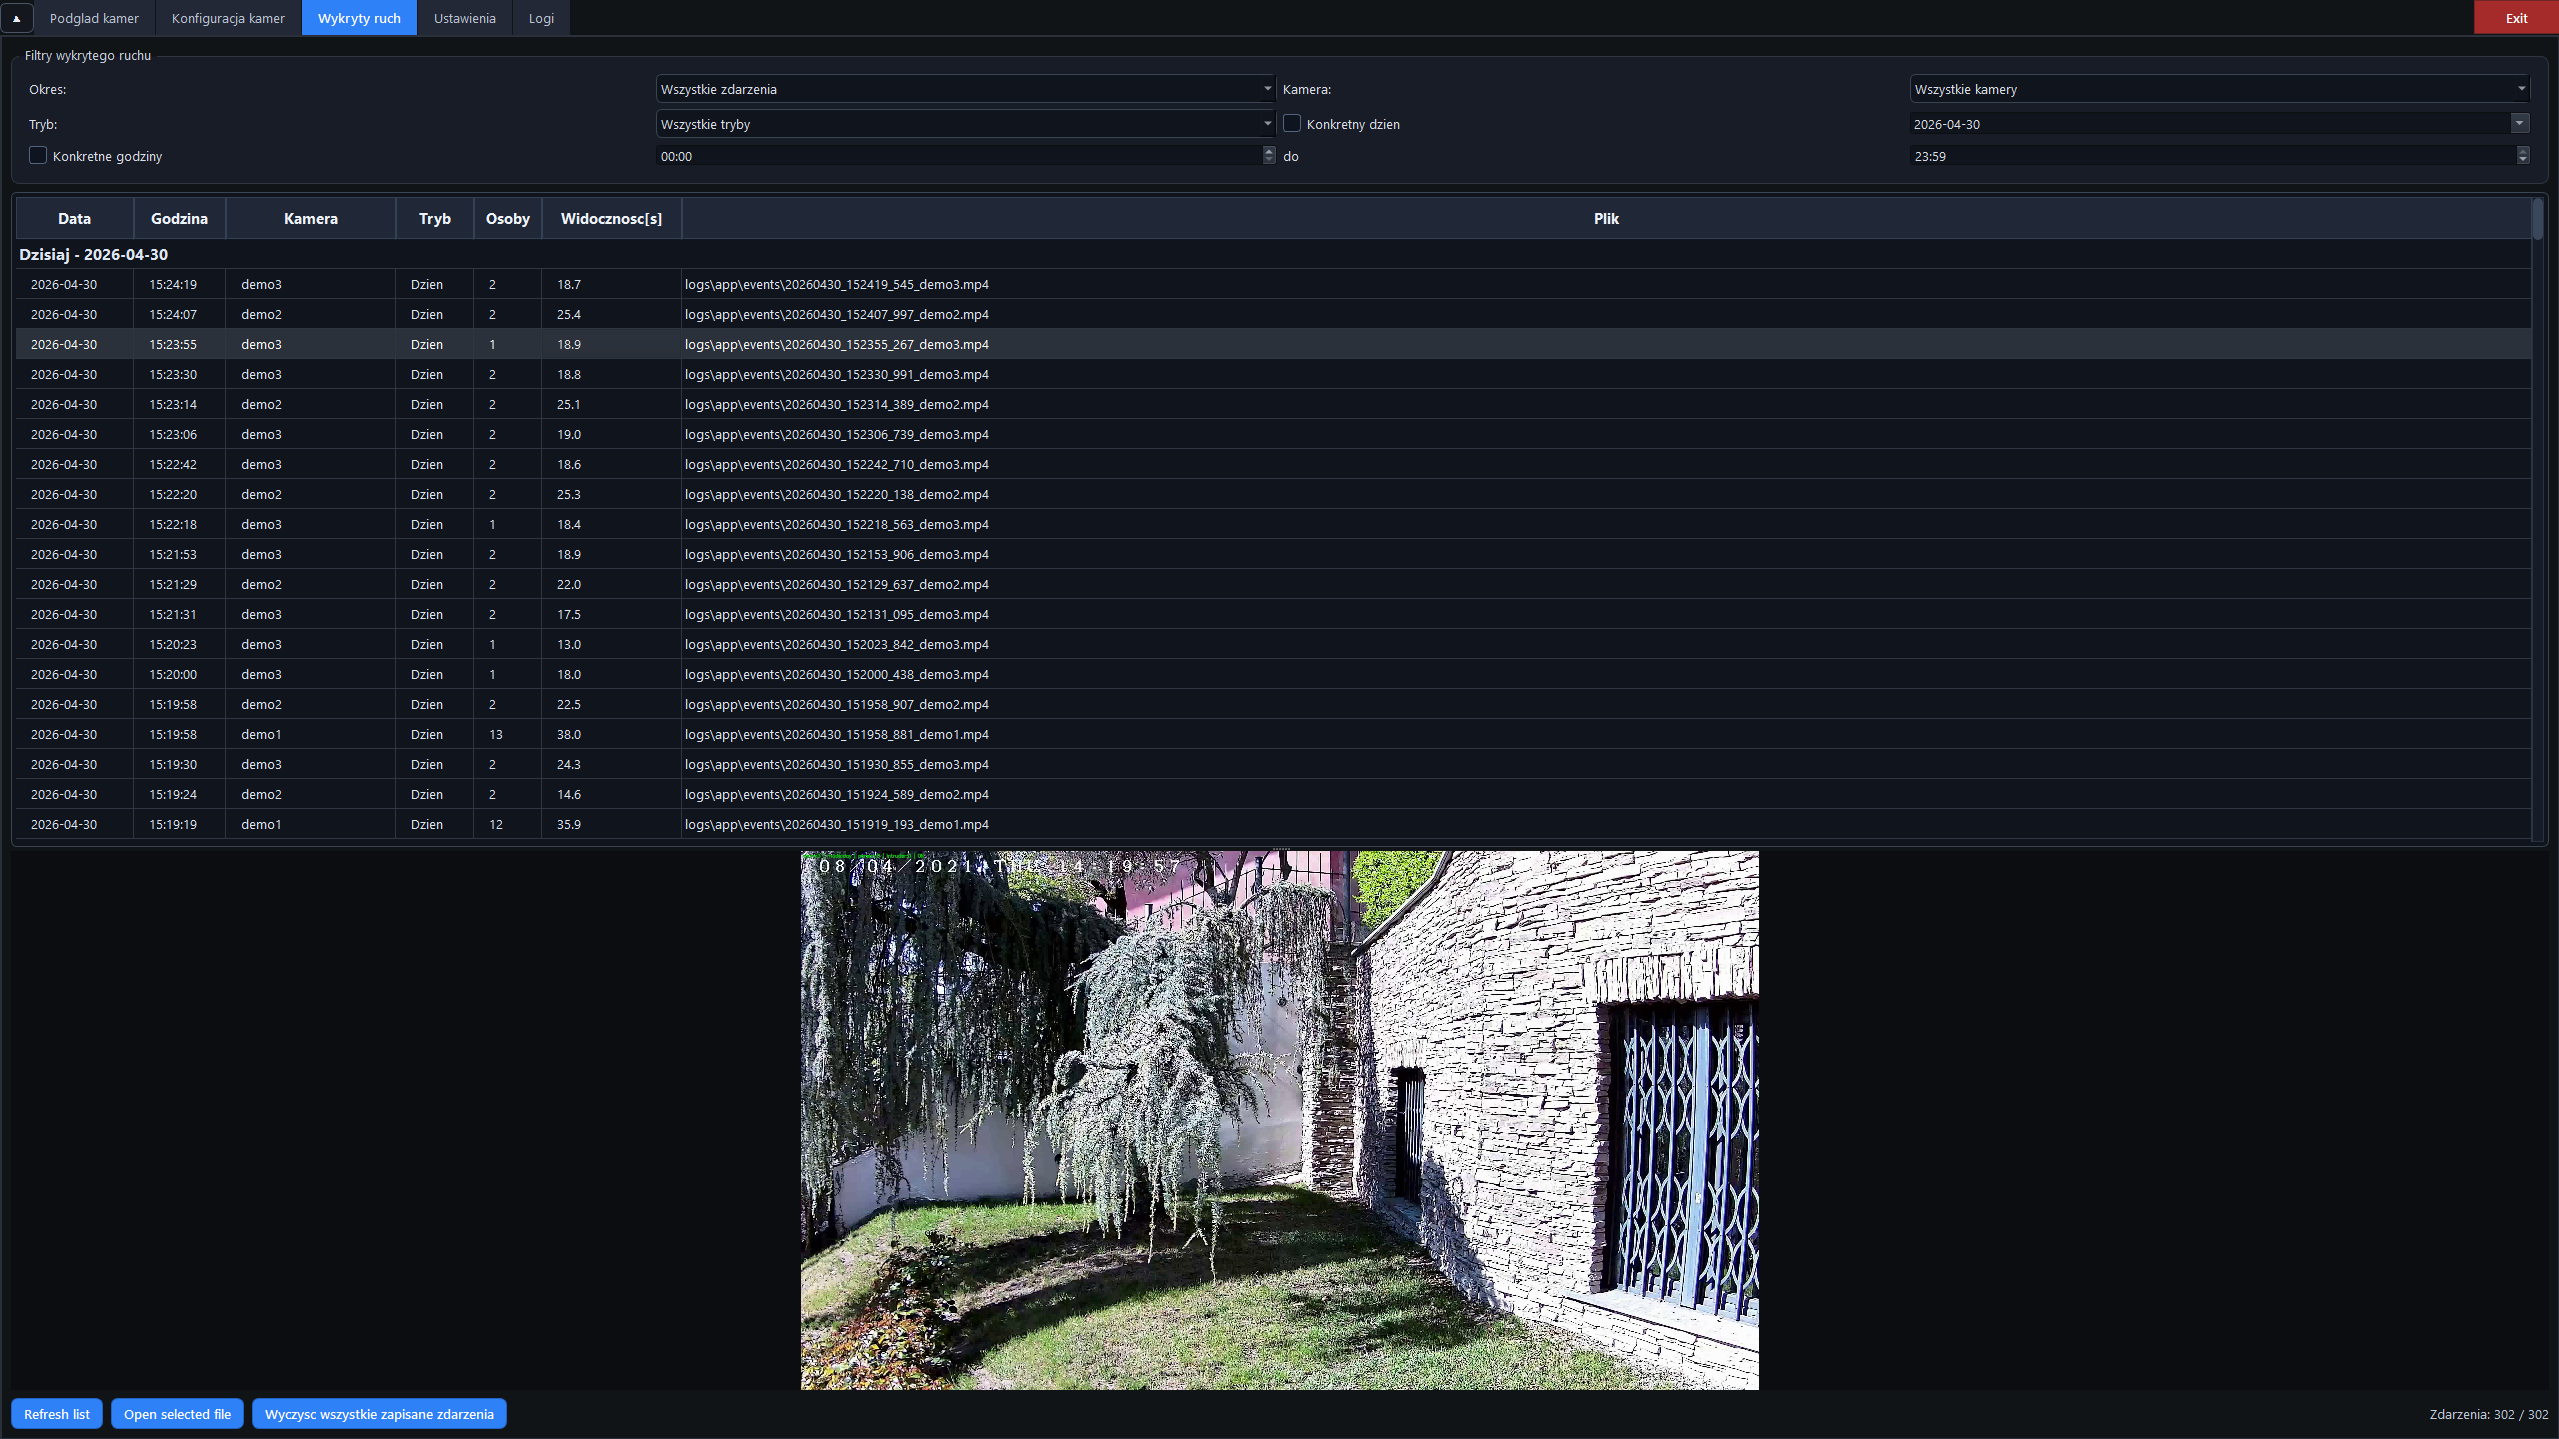
\includegraphics[width=0.95\textwidth]{rys/zakladka-wykryty-ruch.png}
\caption{Historia wykrytego ruchu z filtrowaniem i podglądem zapisanego materiału.}
\label{fig:wykryty-ruch}
\end{figure}

\subsection{Odtwarzacz nagrań i praca z obrazem}

W zakładce podglądu znajduje się również widok nagrań. Operator może wczytać plik wideo, odtworzyć go, zatrzymać, przewinąć suwakiem oraz powiększyć obraz. Podobne mechanizmy zoomu i przesuwania działają w podglądzie kamer na żywo. Pojedynczy kafelek można otworzyć w trybie pełnoekranowym, a wyjście z tego widoku odbywa się za pomocą klawisza \texttt{Esc}, \texttt{F11}, prawego kliknięcia lub przycisku zamknięcia.

\subsection{Presety, logi i obsługa modeli}

Ustawienia aplikacji można zapisywać jako presety i później przywracać. Pozwala to przygotować kilka wariantów pracy, na przykład konfigurację oszczędną, demonstracyjną lub nastawioną na dokładność.

Zakładka ustawień zawiera także katalog modeli YOLO. Aplikacja prezentuje dostępne modele, ich źródło, rozmiar oraz status pobrania. Operator może pobrać wybrany model bez znajomości programowania, a następnie załadować go do działania.

W zakładce logów zapisywane są komunikaty o starcie aplikacji, ładowaniu modeli, zmianach konfiguracji, zapisie zdarzeń oraz błędach runtime. Logi mogą zostać wyeksportowane do pliku, co ułatwia analizę problemów i dokumentowanie testów. Przykład takiej zakładki pokazano na rysunku \ref{fig:logi}.

\begin{figure}[H]
\centering
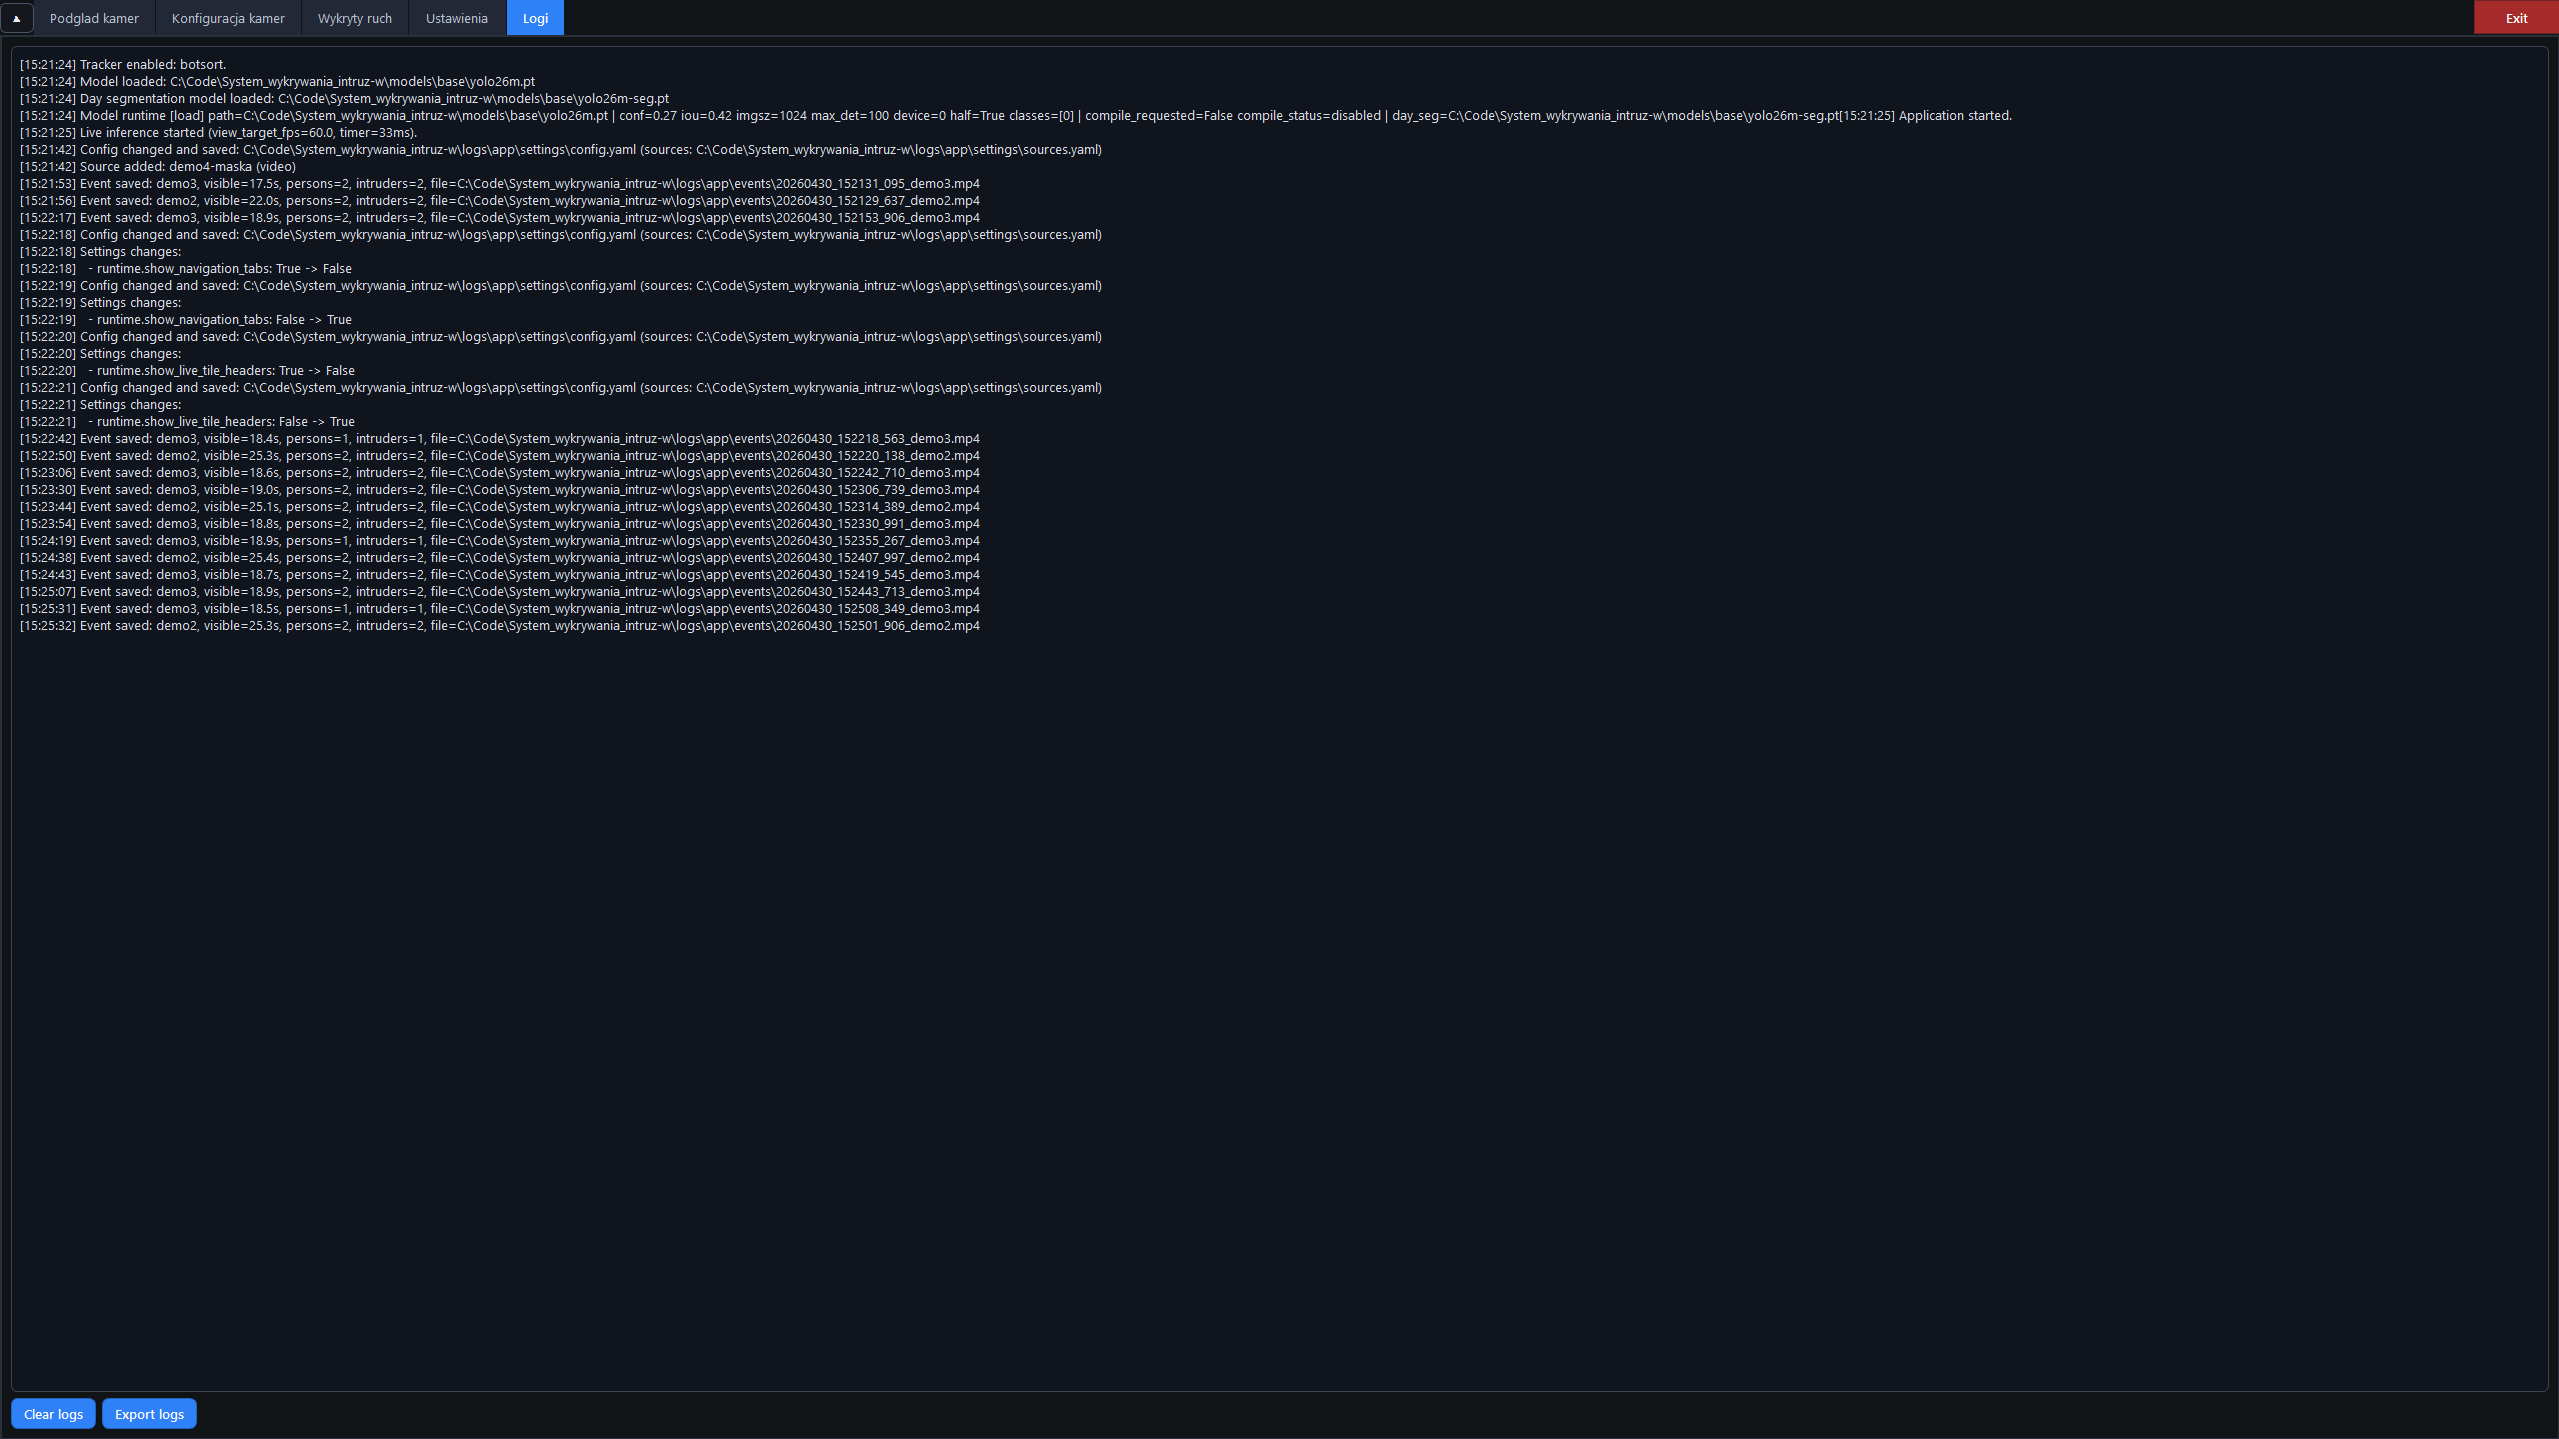
\includegraphics[width=0.95\textwidth]{rys/zakladka-logi.png}
\caption{Zakładka logów aplikacji.}
\label{fig:logi}
\end{figure}
